%!TEX root = ../../main.tex
\section{Experimental methods}
\label{sec:Experimental methods - SAXS}
This section describes the experimental details for two experiments comparing the efficacy of various radioprotectant compounds.
The first of these experiments was carried out in October 2014 whereas the second was carried out in December 2015, both at the ESRF, in Grenoble.

\subsection{Sample preparation}
\label{sub:Sample preparation}
Crystalline glucose isomerase (GI) used in both experiments was purchased in tetrameric form (1552 residues, 172 kDa) from Hampton Research. GI was chosen because it is a stable, soluble globular protein that has well defined SAXS behaviour and is sufficiently large to scatter well at modest concentrations.

\subsubsection{Experiment 1 (Expt 1)}
\label{subs:Experiment 1 - sample prep}
Radioprotectants and GI were dissolved separately in buffer (100$\,$mM HEPES and 10$\,$mM MgCl$_{\text{2}}$ at pH 7.0) to give stock solutions of both at twice the desired radioprotectant and protein concentrations respectively.
The protein and scavenger stocks were then mixed thoroughly by pipetting in a 1:1 ratio to create the samples.
The radioprotectant stock was also mixed in a 1:1 ratio with the buffer by the automatic liquid handling on the beamline to create the buffer sample.
Both samples were prepared at the beamline immediately before the diffraction experiment in order to minimise protein aggregation before data collection.

The final concentrations of each component in solution were as follows:
0.54 mg/ml GI, 5 mM soluble radioprotectant, 5\%$\,$v/v glycerol or ethylene glycol.
Each sample was prepared in triplicate to allow repeats. The following radioprotectants were investigated: sodium ascorbate, sucrose, sodium nitrate, trehalose, ethylene glycol, (2,2,6,6-tetramethylpiperidin-1-yl)oxyl (TEMPO), glycerol and glycerol + nitrate.

\subsubsection{Experiment 2 (Expt 2)}
\label{subs:Experiment 2 - sample prep}
GI was dissolved and dialysed for 24 hours at 277$\,$K with the same buffer components as those used in the first experiment.
The final GI concentration, 1\,mg/ml, used for all data collection runs was determined using the extinction coefficient given by 45,600\,M$^{\text{-1}}$cm$^{\text{-1}}$ at 280\,nm absorbance.
Eight solution additives were tested for their radiation damage protection capabilities: dithiothreitol (DTT), ethylene glycol, glycerol, sodium ascorbate, sodium nitrate, sucrose, (2,2,6,6-tetramethylpiperidin-1-yl)oxyl (TEMPO) and trehalose.
The additives were added to the buffer solutions at four different concentrations: 10$\,$mM, 5$\,$mM, 2$\,$mM and 1$\,$mM, except glycerol and ethylene glycol which were both prepared at 10\%$\,$v/v, 5\%$\,$v/v, 2\%$\,$v/v and 1\%$\,$v/v immediately prior to data collection.
These additives were also prepared to the same final concentration in the solution containing both the buffer and protein.

\subsection{SAXS data collection}
\label{sub:SAXS data collection}

\subsubsection{Experiment 1}
\label{subs:Experiment 1- data col}
Data collection was carried out by Dr. Ed Lowe at the ESRF on beamline BM29.
The X-ray photon energy was 12.5$\,$keV (wavelength of 0.9919 \AA), with a flux of 4.84 $\times$ 10$^{\text{11}}$ photons per second at 100\% transmission.
The size of the beam was 700 $\times$ 700$\,\mu m^{\text{2}}$, however the beam profile was not experimentally measured.
The profile was assumed Gaussian for the purposes of dose calculation (section \ref{sub:Dose calculation}).
Using the EMBL sample loading robot, 15$\,\mu$l of sample was loaded into a 1.8$\,$mm diameter quartz capillary tube with a wall thickness of 0.03$\,$mm and data were collected at 293$\,$K with flow mode turned off.
Frames were collected at 0.5 second intervals on a Pilatus 1M detector for durations of either 30 seconds (60 frames) or 60 seconds (120  frames).

\subsubsection{Experiment 2}
\label{subs:Experiment 2 - data col}
Data collection was performed at the ESRF by the author on beamline BM29 in collaboration with Adam Round and Martha Brennich.
The photon energy used throughout was 12.5$\,$keV and the photon flux was estimated from diode readings which were recorded for every frame using the conversion formula
\begin{equation}
    \text{flux} = \text{5.72293 + 2.72295} \times \text{10}^{\text{15}} \times \text{d}_{\text{r}},
\end{equation}
where d$_{\text{r}}$ is the diode reading.
The flux obtained using this formula was calibrated with an OSD1-0 photodiode purchased from Optoelectronics, which was a 500$\,\mu m$ thick silicon diode with a 1$\,$mm$^{\text{2}}$ active area as per Owen \textit{et al.} (2009) \nocite{owen2009}.
The flux was calculated for each frame because the diode readings constantly changed between frames (Figure~\ref{fig:Diode and flux readings}), however the overall change in diode reading was only 0.54\%.
Despite the small percentage change, account was still taken for this effect in the analysis.
\begin{figure}
    \centering
    \begin{subfigure}[b]{1.0\textwidth}
            \centering
            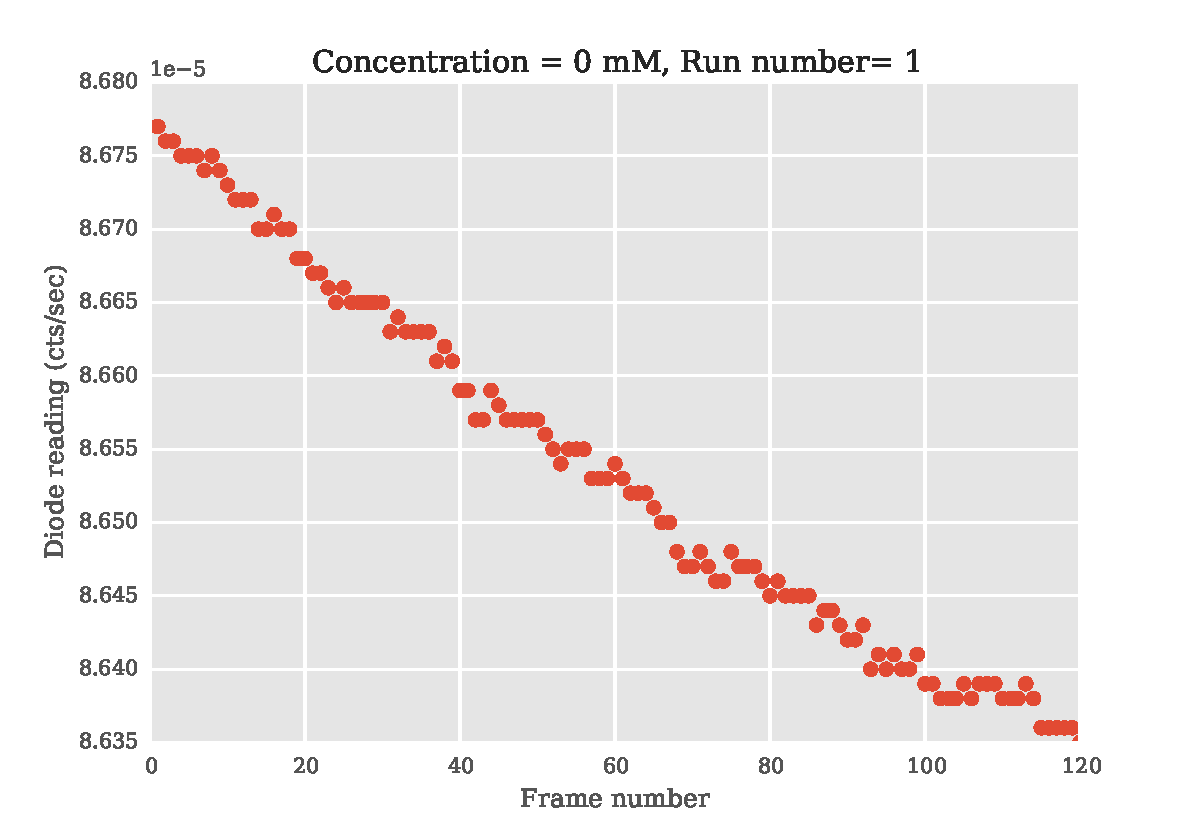
\includegraphics[width=\textwidth]{figures/saxs/np_diode_readings.pdf}
            \caption{}
            \label{fig:Diode readings}
    \end{subfigure}
    \\
    \begin{subfigure}[b]{1.0\textwidth}
            \centering
            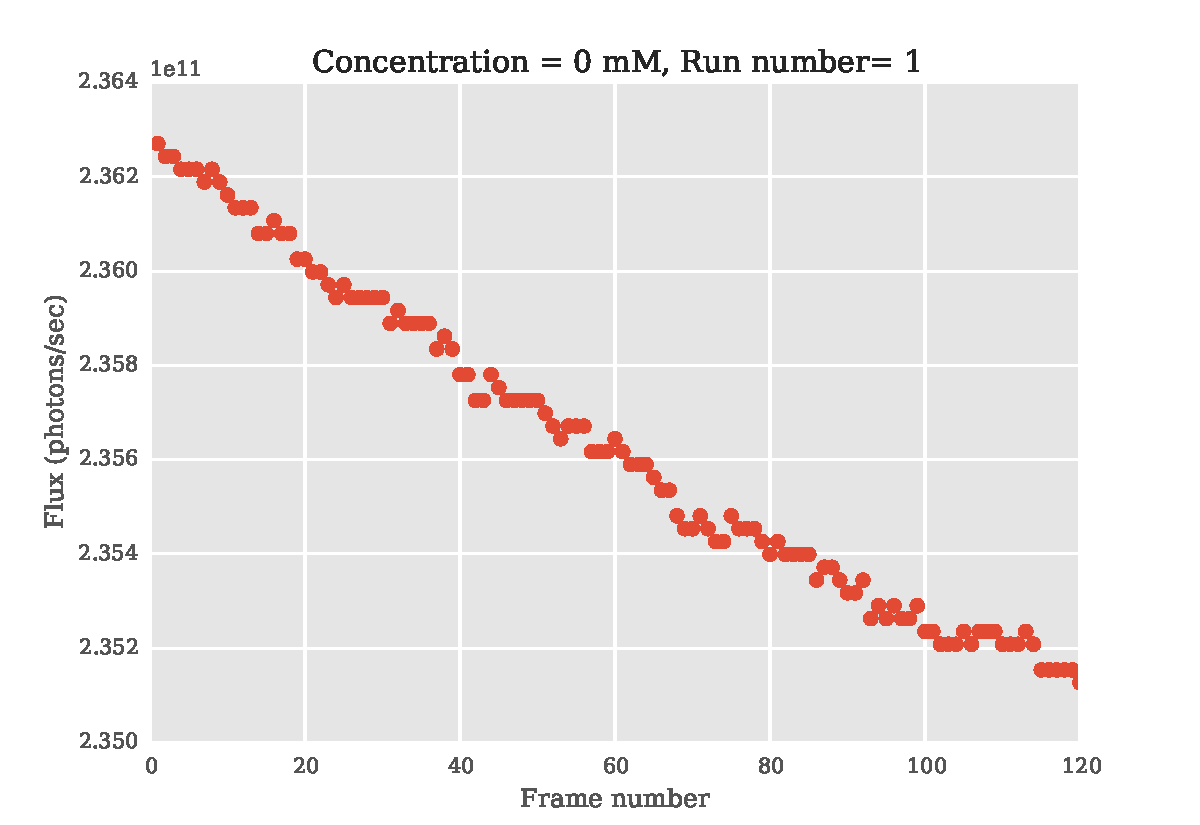
\includegraphics[width=\textwidth]{figures/saxs/np_flux_estimates.pdf}
            \caption{}
            \label{fig:Flux estimates}
    \end{subfigure}
    \caption[Diode readings and flux estimates during the first SAXS repeat for the 1\,mg/ml GI sample with no radioprotecant added.]{Diode readings and flux estimates during the first SAXS repeat for the GI sample with no radioprotecant added (hence concentration = 0\,mM).
    (a) Diode readings for each frame in the experiment.
    It can clearly be seen that the diode readings decrease throughout the experiment, which is due to the decay of the electron storage ring current.
    However, the total change during the course of the dataset is only 0.54\%.
    (b) Flux estimates for each frame in the same experiment as (a).
    As a result of the decreasing diode readings the corresponding flux decreases by 0.54\% too.}
    \label{fig:Diode and flux readings}
\end{figure}
The full 2D X-ray beam profile was determined as outlined in section \ref{sec:Processing multiple 1D aperture scan measurements}. The resulting beam is shown in Figure~\ref{fig:SAXS beam profile} as a greyscale image.
\begin{figure}
    \centering
    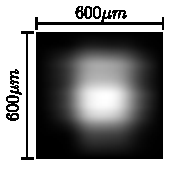
\includegraphics[width=0.6\textwidth]{figures/saxs/SAXS_beam.pdf}
    \caption[A 2D reconstruction of beam used in the second SAXS experiment]{A 2D reconstruction of the beam used in the second SAXS experiment (Expt 2) shown as a greyscale image.}
    \label{fig:SAXS beam profile}
\end{figure}

The data were recorded using a Pilatus 1M detector from Dectris.
15\,$\mu l$ of each sample was loaded into a 1.8$\,$mm external diameter quartz capillary (1.7\,mm internal diameter, thus the wall thickness is 50\,$\mu m$) held at room temperature using the automated robotic sample changer \cite{round2015biosaxs}.
For each additive, data were collected at each concentration (given in section \ref{sub:Sample preparation}), and each of these runs was repeated 3 times.
The exposure time for each frame was 1 second, and a total of 120 frames were collected for a single run with the sample kept static.
For each radioprotecant concentration a single dataset was collected with only the buffer (no protein) so that a suitable buffer correction (subtraction) could be applied during data analysis.

\subsection{Dose calculations}
\label{sub:Dose calculation}
Dose calculations for both experiments were performed using RADDOSE-3D with the modifications described in section \ref{sec:Extending RADDOSE-3D for SAXS} for modelling SAXS experiments.
An example input file for Expt 1 can be seen in Figure~\ref{fig:SAXS example input - Rebecca}.
The beam profile was assumed Gaussian with full width at half maximum of 110$\,\mu m \times $200$\,\mu m$.
\begin{figure}
    \centering
    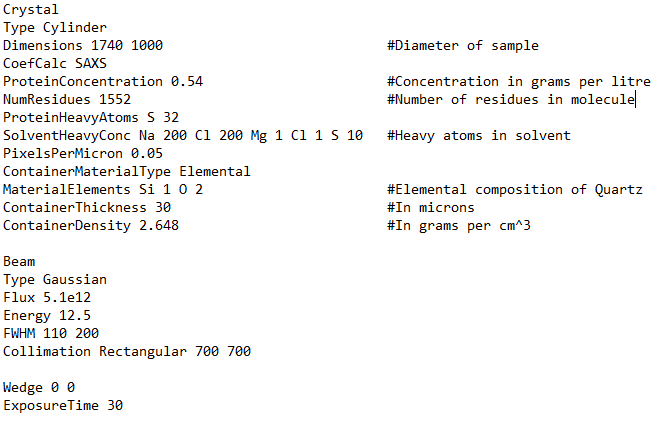
\includegraphics[width=0.7\textwidth]{figures/saxs/rebecca_raddose_input.png}
    \caption[RADDOSE-3D input file used for the dose calculations in Expt 1.]{RADDOSE-3D input file used for the dose calculations in Expt 1.}
    \label{fig:SAXS example input - Rebecca}
\end{figure}
For Expt 2, the beam image shown in Figure~\ref{fig:SAXS beam profile} was read directly into RADDOSE-3D and the corresponding flux values recorded for each frame were used to ensure accurate dose estimates.
The atomic composition is the same as that defined in Figure~\ref{fig:SAXS example input - Rebecca}, although the 5\,mM concentration of sodium is only defined for the radioprotectants that contain sodium (i.e. sodium ascorbate and sodium nitrate).
DTT contains a sulphur atom for which account must be taken also in the solvent concentration.
The elemental composition of the quartz capillary was entered into RADDOSE-3D as SiO$_{\text{2}}$.
The capillary thickness was given as 50$\,\mu m$ and a density of 2.648$\,$g/cm$^{\text{3}}$ was used.
